
\documentclass[pdflatex,sn-mathphys-num]{sn-jnl}% Math and Physical Sciences Numbered Reference Style 
%%\documentclass[pdflatex,sn-mathphys-ay]{sn-jnl}% Math and Physical Sciences Author Year Reference Style
%%\documentclass[pdflatex,sn-aps]{sn-jnl}% American Physical Society (APS) Reference Style
%%\documentclass[pdflatex,sn-vancouver,Numbered]{sn-jnl}% Vancouver Reference Style
%%\documentclass[pdflatex,sn-apa]{sn-jnl}% APA Reference Style 
%%\documentclass[pdflatex,sn-chicago]{sn-jnl}% Chicago-based Humanities Reference Style

%%%% Standard Packages
%%<additional latex packages if required can be included here>
\usepackage{epstopdf}
\usepackage{graphicx}%
\usepackage{multirow}%
\usepackage{amsmath,amssymb,amsfonts}%
\usepackage{amsthm}%
\usepackage{mathrsfs}%
\usepackage[title]{appendix}%
\usepackage{xcolor}%
\usepackage{textcomp}%
\usepackage{manyfoot}%
\usepackage{booktabs}%
\usepackage{algorithm}%
\usepackage{algorithmicx}%
\usepackage{algpseudocode}%
\usepackage{listings}%
\usepackage{tabularx}
\usepackage{float}


%%%%

%%%%%=============================================================================%%%%
%%%%  Remarks: This template is provided to aid authors with the preparation
%%%%  of original research articles intended for submission to journals published 
%%%%  by Springer Nature. The guidance has been prepared in partnership with 
%%%%  production teams to conform to Springer Nature technical requirements. 
%%%%  Editorial and presentation requirements differ among journal portfolios and 
%%%%  research disciplines. You may find sections in this template are irrelevant 
%%%%  to your work and are empowered to omit any such section if allowed by the 
%%%%  journal you intend to submit to. The submission guidelines and policies 
%%%%  of the journal take precedence. A detailed User Manual is available in the 
%%%%  template package for technical guidance.
%%%%%=============================================================================%%%%

%% as per the requirement new theorem styles can be included as shown below
\newtheorem{theorem}{Theorem}%  meant for continuous numbers
%%\newtheorem{theorem}{Theorem}[section]% meant for sectionwise numbers
%% optional argument [theorem] produces theorem numbering sequence instead of independent numbers for Proposition
\newtheorem{proposition}[theorem]{Proposition}% 
%%\newtheorem{proposition}{Proposition}% to get separate numbers for theorem and proposition etc.

\newtheorem{example}{Example}%
\newtheorem{remark}{Remark}%

\newtheorem{definition}{Definition}%

\raggedbottom
%%\unnumbered% uncomment this for unnumbered level heads

\begin{document}

\title[Article Title]{Optimizing Information Retrieval: A Hybrid Model Leveraging MAR and RAPTOR Frameworks}

%%=============================================================%%
%% GivenName	-> \fnm{Joergen W.}
%% Particle	-> \spfx{van der} -> surname prefix
%% FamilyName	-> \sur{Ploeg}
%% Suffix	-> \sfx{IV}
%% \author*[1,2]{\fnm{Joergen W.} \spfx{van der} \sur{Ploeg} 
%%  \sfx{IV}}\email{iauthor@gmail.com}
%%=============================================================%%

\author[1]{\fnm{Timur} \sur{Abdygulov}}\email{timur.abdygulov@gwu.edu}



\author*[2]{\fnm{Amir H.} \sur{Jafari}}\email{ajafari@email.gwu.edu}
%\equalcont{These authors contributed equally to this work.}

\affil*[1,2]{\orgdiv{Data Science}, \orgname{George Washington University}, \orgaddress{\street{2121 I St NW}, \city{Washington, DC}, \postcode{20052}, \state{State}, \country{United States of America}}}



\abstract{The proliferation of unstructured data has exposed the limitations of traditional retrieval systems in addressing complex queries, \emph{multi-hop reasoning}, and context-aware synthesis. This study evaluates four Retrieval-Augmented Generation (RAG) systems—Naive RAG, Memory-Augmented Retrieval (MAR), Recursive Abstractive Processing for Tree-Organized Retrieval (RAPTOR), and a novel Hybrid Model—using the BioASQ biomedical dataset. MAR leverages memory persistence to excel in static queries but struggles with \emph{dynamic adaptability}. RAPTOR employs \emph{hierarchical abstraction} to enhance \emph{multi-hop reasoning} but lacks \emph{persistent memory} capabilities. The Hybrid Model integrates MAR’s \emph{memory-driven retrieval} with RAPTOR’s hierarchical reasoning to balance performance across query types, achieving superior results in both static and dynamic tasks. Key findings emphasize the critical role of embedding strategies in retrieval performance and highlight avenues for advancing query refinement, adaptive retrieval techniques, and \emph{multimodal integration}. These innovations aim to address scalability and contextual understanding challenges, positioning the Hybrid Model as a robust framework for context-aware, scalable information retrieval.}


\keywords{Retrieval-Augmented Generation (RAG), Memory-Augmented Retrieval (MAR), Hierarchical Retrieval, Biomedical Information Retrieval, \emph{multi-hop reasoning}, Hybrid Model}


\maketitle

\section{Introduction}\label{sec1}
The rapid proliferation of unstructured data has posed significant challenges to traditional information retrieval systems, particularly in synthesizing meaningful insights from extensive and complex contexts. \emph{Retrieval-Augmented Generation (RAG)} frameworks have emerged as a transformative approach, dynamically integrating retrieval mechanisms with large language models (LLMs) to enhance \emph{contextual relevance}, reasoning capabilities, and response accuracy. Over the past decade, RAG systems have significantly evolved, moving from naive implementations that integrate static retrieval with generation to sophisticated models that incorporate memory hierarchies, hybrid retrieval strategies, and \emph{adaptive optimization}.

Among the foundational advancements, MemoRAG introduces memory hierarchies and \emph{dynamic updates} to improve \emph{retrieval efficiency} and precision, addressing the limitations of static retrieval systems in dynamic environments \cite{bib1}. Similarly, RAPTOR organizes data into hierarchical tree structures for multi-level context aggregation and recursive reasoning, making it particularly effective for multi-hop question answering and abstractive summarization \cite{bib2}. Early implementations like MemLong extend RAG capabilities by leveraging long-context modeling and hierarchical indexing to efficiently manage ultra-long contexts, while LONGMEM further enhances retrieval consistency by mitigating memory staleness through decoupled memory architectures \cite{bib3, bib4}. Complementing these is MemReasoner, which builds on temporal reasoning and iterative refinement to improve \emph{multi-hop reasoning} over complex datasets \cite{bib5}.

Hybrid models have further advanced the field by addressing challenges related to scalability, adaptability, and retrieval precision. Blended RAG employs hybrid query strategies, combining dense and sparse vector retrieval techniques to optimize performance across diverse datasets like NQ and TREC-COVID \cite{bib6}. MBA-RAG dynamically adjusts retrieval strategies using a multi-armed bandit framework, achieving a balance between efficiency and accuracy in complex queries \cite{bib7}. HIRO introduces recursive similarity scoring and hierarchical pruning to improve scalability for large-scale datasets, while LightRAG uses graph-structured indexing and dual-level retrieval to enhance the synthesis of interdependent data \cite{bib8, bib9}.

Sophisticated frameworks such as HybridRAG and RAG Foundry extend RAG capabilities by integrating structured relational data with unstructured semantic information, improving retrieval workflows and enhancing contextual coherence in generated outputs \cite{bib10, bib11}. Additionally, COCOM introduces a context compression model that reduces inference time while preserving generative quality, significantly advancing \emph{retrieval efficiency} in multi-document QA tasks \cite{bib12}. ContextRAG complements these innovations by refining query-sensitive retrieval methods to improve relevance for contextually dependent tasks \cite{bib13}. In domain-specific applications, BootHealthCare LLM optimizes retrieval pipelines for healthcare-related queries, demonstrating its utility in enhancing factual reliability in open-ended question answering \cite{bib19}.

Other approaches emphasize adaptability and retrieval optimization. Retrieve Anything and ADAPT-LLM provide versatile retrievers that dynamically adapt to both external and internal knowledge requirements, ensuring consistent relevance in diverse retrieval scenarios \cite{bib14, bib15}. The MAR Mixture of Word Experts framework introduces sparse architectures tailored for knowledge-intensive NLP tasks, achieving a balance between computational efficiency and task-specific performance \cite{bib20}. Additionally, studies like Text Embeddings Reveal highlight the potential of embeddings to recover semantic-rich information while addressing concerns of privacy and robustness in retrieval systems \cite{bib16}.

Several frameworks explore iterative and evidence-supported generation. The Active Retrieval Augmented Generation (ARAG) framework ensures forward-looking, knowledge integration for \emph{multi-hop reasoning}, while Understanding Retrieval Augmentation for Long QA emphasizes evidence attribution and contextual coherence in generating long-form responses \cite{bib17, bib18}. Practical insights from Searching for Best RAG Methods provide guidance on selecting optimal retrieval techniques for diverse applications \cite{bib21}, while When to Retrieve focuses on the timing of retrieval and its impact on query relevance, offering strategies to improve system adaptability and performance \cite{bib22}.

This paper primarily builds on MemoRAG, RAPTOR, and Naive RAG as foundational frameworks, which serve as core elements in developing the MAR, RAPTOR, and Hybrid models discussed herein. MemoRAG’s memory hierarchies, RAPTOR’s hierarchical context organization, and Naive RAG’s straightforward retrieval-generation integration provide the foundational structure for these advanced models. By extending these frameworks with targeted innovations, such as adaptive retrieval strategies, \emph{hierarchical abstraction}, and \emph{multi-hop reasoning}, this paper proposes solutions to key challenges in retrieval-augmented generation. The resulting models emphasize dynamic retrieval, contextual coherence, and scalable performance, offering robust solutions for complex information retrieval tasks.


\section{Problem Statement}\label{sec2}
Traditional retrieval systems face significant inefficiencies when addressing tasks that require extensive contextual understanding, precise query resolution, and \emph{multi-hop reasoning}. \emph{token constraints} in language models hinder their ability to handle ultra-long contexts, resulting in incomplete or fragmented responses. Additionally, these systems lack mechanisms to refine ambiguous inputs into actionable queries, and they struggle to synthesize evidence across distributed sources, further exposing their limitations in \emph{dynamic adaptability} and complex reasoning.

Existing RAG frameworks attempt to address these challenges but remain constrained in scope. Memory-Augmented Retrieval (MAR) enhances performance in static query handling through memory persistence but lacks adaptability for dynamic or multi-layered tasks. Conversely, Recursive Abstractive Processing for Tree-Organized Retrieval (RAPTOR) excels at \emph{multi-hop reasoning} with hierarchical data organization but fails to incorporate \emph{persistent memory}, limiting its efficacy in recalling historical or infrequently accessed information.

Recent advancements demonstrate the potential for integrating long-context modeling with hierarchical indexing to manage ultra-long inputs effectively and highlight the benefits of combining \emph{vector-based retrieval} with knowledge graphs, improving domain-specific query handling. Other innovations address various aspects of retrieval challenges, including dynamic strategy optimization, hybrid query processing, and recursive abstraction.

Despite these advancements, existing systems still exhibit trade-offs between \emph{static memory recall} and dynamic reasoning capabilities. To overcome these limitations, this study proposes a Hybrid Model that integrates MAR’s memory persistence and RAPTOR’s \emph{hierarchical abstraction} while incorporating features from state-of-the-art frameworks. The Hybrid Model aims to deliver a scalable, context-aware solution capable of addressing the challenges of both static and dynamic query scenarios.


\section{Methodology}\label{sec3}
This study evaluates four Retrieval-Augmented Generation (RAG) systems—Naive RAG, Memory-Augmented Retrieval (MAR), Recursive Abstractive Processing for Tree-Organized Retrieval (RAPTOR), and the Hybrid Model—using a modular and extensible framework. Each system integrates a retrieval mechanism interfacing with a vector store for \emph{semantic similarity searches} and a generative language model for synthesizing query-relevant responses.

\subsection{Retrieval-Augmented Generation (Naive RAG)}\label{subsec2}
Naive RAG forms the baseline, implementing a straightforward two-phase process: retrieval and generation. Queries are embedded into a high-dimensional vector space and matched against pre-indexed embeddings in the vector store using semantic similarity. Top-k documents are retrieved and passed to a generative language model for response synthesis. Preprocessing involves chunking documents into fixed-size text segments with overlapping characters to preserve context. Figure 1 illustrates the Naive RAG workflow.

\begin{figure}[h]
    \centering
    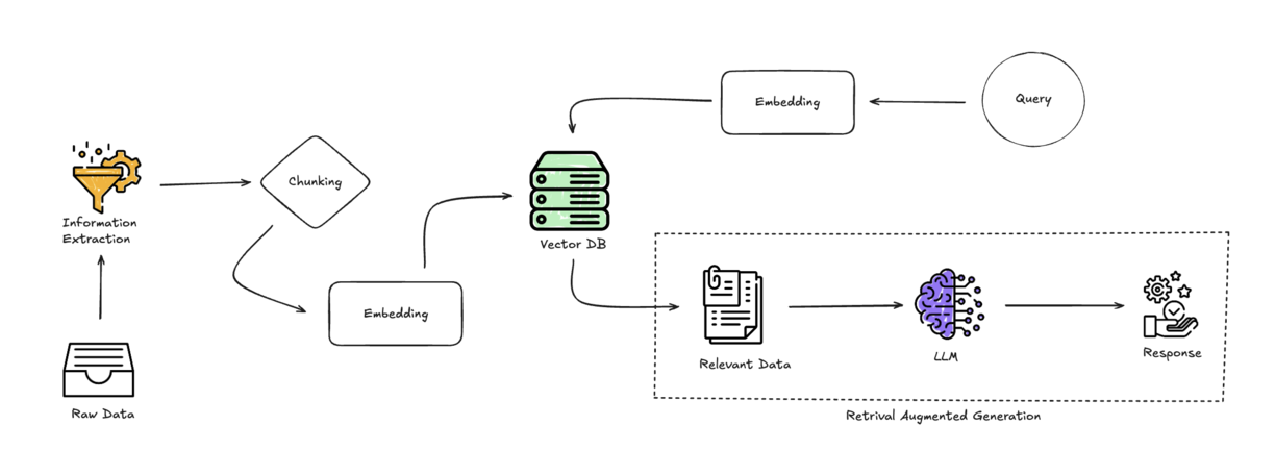
\includegraphics[width=0.8\textwidth]{Basic_Rag.eps}
    \caption{Basic workflow of a Retrieval-Augmented Generation (RAG) system.}
    \label{fig:rag_pipeline}
\end{figure}


\subsection{Memory-Augmented Retrieval (MAR)}\label{subsec2}
MAR extends Naive RAG by incorporating a MemoryDB for handling static, frequently recurring queries. A similarity threshold determines if the query matches an entry in MemoryDB; if not, retrieval falls back to vector-based methods. This approach ensures efficiency for static tasks but limits adaptability to dynamic contexts. Figure 2 highlights the MAR architecture.

\begin{figure}[h]
    \centering
    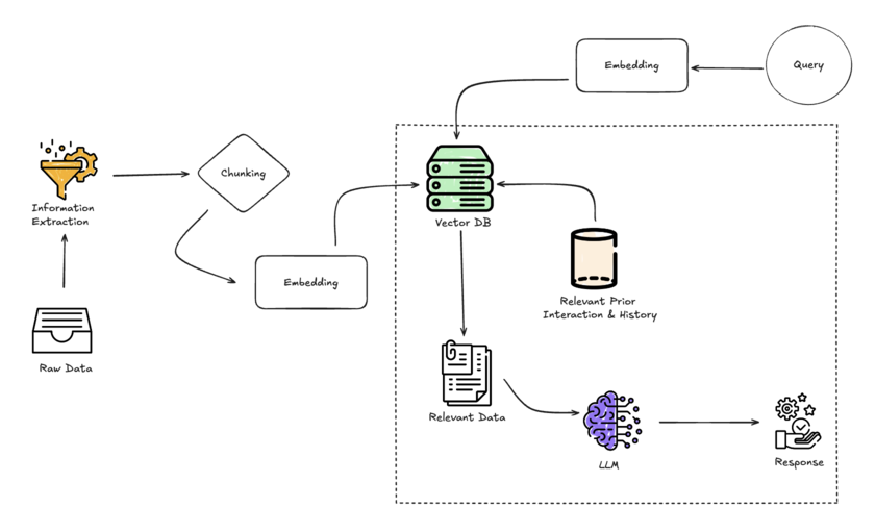
\includegraphics[width=0.6\textwidth]{MAR_rag.eps}
    \caption{Workflow of the Memory-Augmented Retrieval (MAR) system.}
    \label{fig:mar_pipeline}
\end{figure}    


\subsection{Recursive Abstractive Processing for Tree-Organized Retrieval (RAPTOR)}\label{subsec2}
RAPTOR organizes documents hierarchically using semantic clustering and recursive abstraction. This method supports \emph{multi-hop reasoning}, as queries traverse semantic clusters. While advanced clustering methods like UMAP or GMM are common, this study employs quantization to reduce computational complexity. Figure 3 showcases RAPTOR’s hierarchical structure.


\begin{figure}[h]
    \centering
    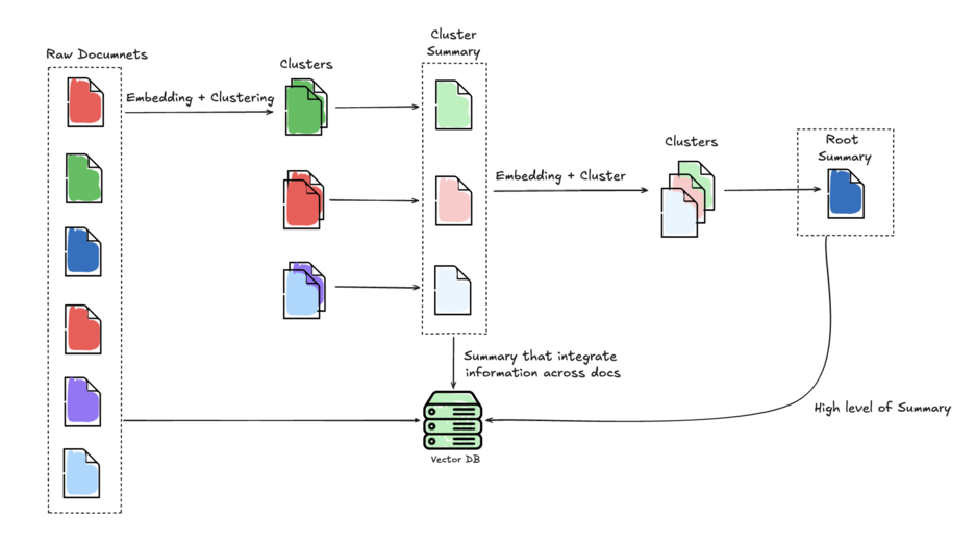
\includegraphics[width=0.8\textwidth]{RAPTOR_rag.eps}
    \caption{Hierarchical retrieval architecture of the RAPTOR system.}
    \label{fig:raptor_pipeline}
\end{figure}


\subsection{The Hybrid Model}\label{subsec2}
The Hybrid Model combines MAR’s \emph{memory-driven retrieval} with RAPTOR’s \emph{hierarchical abstraction}, enabling balanced performance across static and dynamic tasks. Queries are routed through MAR or RAPTOR based on a dynamic similarity threshold, optimizing retrieval processes. MemoryDB handles recurring queries, while RAPTOR processes \emph{multi-hop reasoning} tasks. Figure 4 depicts the Hybrid Model’s architecture.

\begin{figure}[h]
    \centering
    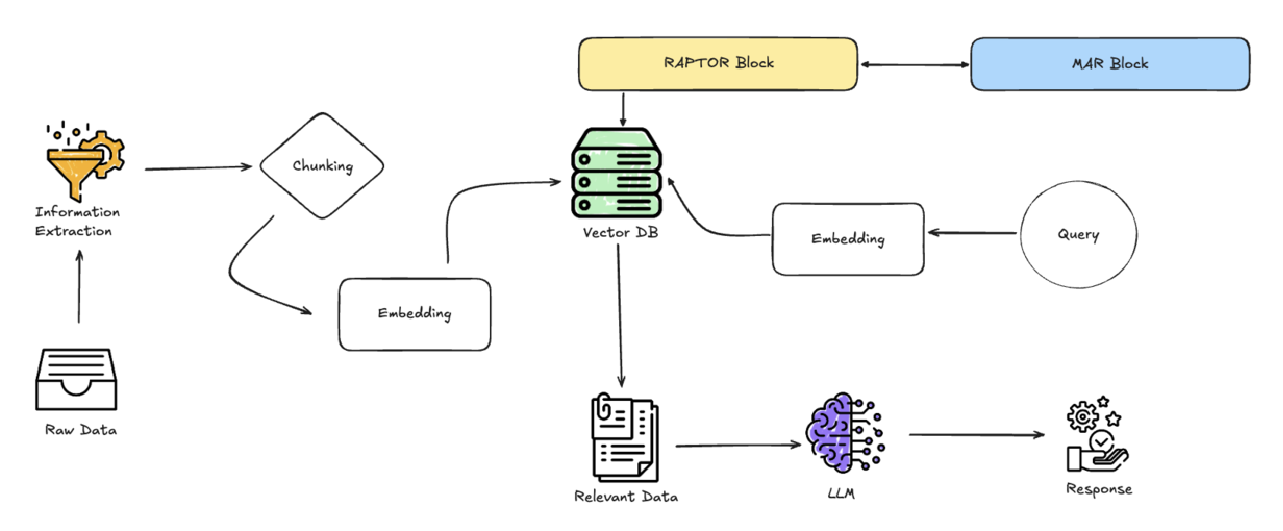
\includegraphics[width=0.8\textwidth]{HYBRID_rag.eps}
    \caption{Architecture of the Hybrid Model, combining MAR and RAPTOR systems.}
    \label{fig:hybrid_pipeline}
\end{figure}


\subsection{Retrieval System: ChromaDB}\label{subsec2}
ChromaDB serves as the vector store due to its scalability, low-latency query processing, and support for high-dimensional embeddings. It integrates seamlessly with frameworks like LangChain and embedding models such as mxbai-embed-large. ChromaDB's ability to handle hybrid retrieval methods ensures adaptability to both semantic and keyword-based search scenarios.


\subsection{Model Configuration and Hyper-parameters}\label{subsec2}
The models share foundational hyperparameters for preprocessing and embedding generation. Key configurations include:
\begin{itemize}
    \item \textbf{Chunk size}: Defines the maximum text length for document segmentation.
    \item \textbf{Chunk overlap}: Ensures contextual continuity across consecutive chunks.
    \item \textbf{Embedding dimensions}: Standardized to align with vector store requirements.
    \item \textbf{Batch size}: Optimized for embedding generation and indexing.
\end{itemize}


\begin{table}[h]
\caption{Hyperparameters and their descriptions}\label{tab1}%
\begin{tabular}{@{}p{0.2\textwidth}p{0.15\textwidth}p{0.6\textwidth}@{}}
\toprule
\textbf{Hyperparameter} & \textbf{Value/Default} & \textbf{Description} \\
\midrule
chunk\_size & 1000 & The maximum size of text chunks for splitting documents. \\
chunk\_overlap & 115 & The number of overlapping characters between consecutive text chunks. \\
embedding\_dim & 1024 & Dimension of the embeddings generated by the model. \\
batch\_size & 16 (embedding), 50 (indexing) & Batch size for document processing during embedding generation or indexing. \\
\botrule
\end{tabular}
\end{table}

The Hybrid Model introduces additional configurations tailored to its architecture, such as dynamic similarity thresholds, reranking strategies, and memory cache limits. These hyperparameters govern the balance between \emph{memory-driven retrieval} and \emph{hierarchical abstraction}. Details for shared parameters are presented in Table 1, while Table A1 (provided in the Appendix) outlines the specific configurations for the Hybrid Model, including:
\begin{itemize}
    \item \textbf{Dynamic similarity thresholds}: Ranges for adaptive query routing.
    \item \textbf{Reranking top-k}: Specifies the number of retrieved results for reranking.
    \item \textbf{Compression levels}: Applied to optimize embedding storage.
\end{itemize}

These tables collectively highlight the careful design and parameter optimization underpinning the system's performance.


\subsection{Dataset Description}\label{subsec2}
This study uses the BioASQ biomedical dataset \cite{bib23}, a well-established benchmark for evaluating information retrieval systems. Figure 5, describes the Data preparation steps. The dataset comprises diverse biomedical queries that were categorized into three types:
\begin{itemize}
    \item \textbf{Static (S)}: Straightforward factual questions.
    \item \textbf{Dynamic (D)}: Queries requiring updated or evolving contextual information.
    \item \textbf{Multi-layered (M)}: Questions involving \emph{multi-hop reasoning} or evidence synthesis across multiple sources.
\end{itemize}

\begin{figure}[h]
    \centering
    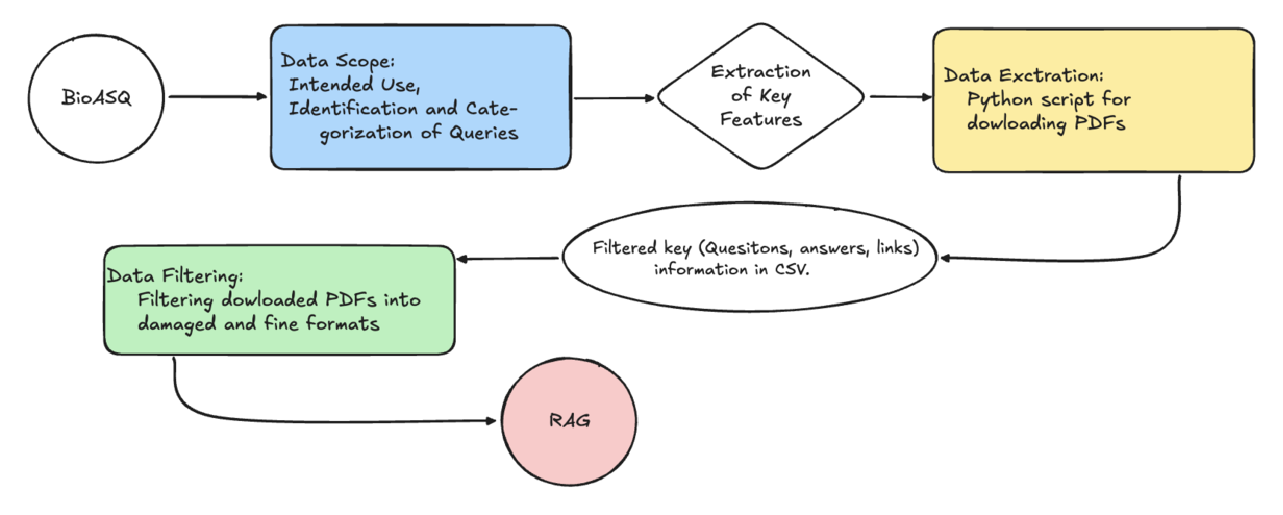
\includegraphics[width=0.8\textwidth]{Dataset_Diagram.eps}
    \caption{Processing Dataset diagram}
    \label{fig:Dataset_Diagram}
\end{figure}

Table 3 provides examples of categorized biomedical queries, illustrating the range of complexity evaluated in this study. Ground truth answers, derived from authoritative sources such as PubMed, served as benchmarks for assessing system performance.

\begin{table}[h]
\caption{Categorized Biomedical Queries}\label{tab:questions_categories}%
\begin{tabular}{@{}p{0.05\textwidth}p{0.65\textwidth}p{0.2\textwidth}@{}}
\toprule
\textbf{ID} & \textbf{Question} & \textbf{Category} \\
\midrule
1 & Is Hirschsprung disease a Mendelian or a multifactorial disorder? & M \\
2 & List signaling molecules (ligands) that interact with the receptor EGFR? & S \\
3 & Are long non-coding RNAs spliced? & M \\
4 & Is RANKL secreted from the cells? & S \\
5 & Which miRNAs could be used as potential biomarkers for epithelial ovarian cancer? & M \\
6 & Which acetylcholinesterase inhibitors are used for treatment of myasthenia gravis? & S \\
7 & Has Denosumab (Prolia) been approved by FDA? & D \\
8 & Which are the different isoforms of the mammalian Notch receptor? & S \\
9 & Orteronel was developed for treatment of which cancer? & D \\
10 & Is the monoclonal antibody Trastuzumab (Herceptin) of potential use in the treatment of prostate cancer? & D \\
11 & Which are the Yamanaka factors? & S \\
12 & Where is the protein Pannexin1 located? & S \\
13 & Which currently known mitochondrial diseases have been attributed to POLG mutations? & M \\
\botrule
\end{tabular}
\end{table}

During preprocessing, the dataset underwent thorough cleaning to resolve issues such as inconsistent formats and inaccessible PDFs. Despite these efforts, some documents linked to the dataset could not be retrieved due to damaged or missing files. Table 4 summarizes the frequency of successfully retrieved PDFs for each query, highlighting variations in data availability that influenced evaluation outcomes.

\section{Relevance}\label{sec4}
The categorization of queries into static, dynamic, and multi-layered types reflects the diversity and complexity of biomedical information retrieval tasks. These categories allow for a comprehensive evaluation of the systems’ performance, testing their capabilities in memory recall, contextual adaptability, and \emph{multi-hop reasoning}. This classification ensures that the study rigorously assesses the strengths and limitations of each retrieval-augmented generation system.


\section{Results}\label{sec5}
The evaluations of MAR, RAPTOR, and the Hybrid Model were conducted on an AWS g5.2xlarge instance, chosen for its compatibility with GPU-based computations and support for large-scale models. This instance, equipped with one NVIDIA A10G Tensor Core GPU, 8 vCPUs, and 32 GiB of memory, provided the necessary \emph{computational resources} for running retrieval tasks, embedding evaluations, and memory optimization. The use of 8-bit precision loading for embedding models further optimized GPU memory usage, enabling the efficient execution of large-scale experiments.

\subsection{System Performance Across Querie}\label{subsec2}
The performance of Naive RAG, MAR, RAPTOR, and the Hybrid Model was evaluated on static, dynamic, and multi-layered queries from the BioASQ dataset. These queries, categorized by their complexity, tested each system’s ability to handle memory recall, \emph{contextual reasoning}, and multi-hop synthesis.

\textbf{Naive RAG}: Naive RAG operates on a straightforward retrieval-to-generation pipeline. While effective for simple factual queries, it struggles with dynamic and multi-layered contexts due to its lack of memory and hierarchical reasoning capabilities. Examples of its performance are presented in Table 1: Naive-Rag. Answer \& Query Results.
\begin{table}[h]
\caption{Naive-Rag. Answer \& Query results}\label{tab:naive_rag_results}%
\begin{tabular}{@{}p{0.3\textwidth}p{0.25\textwidth}p{0.25\textwidth}p{0.1\textwidth}@{}}
\toprule
\textbf{Question} & \textbf{Ideal Answer} & \textbf{Naive RAG Answer} & \textbf{Result} \\
\midrule
What is acetylcholinesterase used for? & Acetylcholinesterase breaks down acetylcholine. & Acetylcholinesterase breaks down acetylcholine. &  Correct \\
Has Denosumab (Prolia) been approved by FDA? & Yes, approved by the FDA in 2010. & No information available. & Incorrect \\
\botrule
\end{tabular}
\end{table}

\textbf{MAR}: MAR enhances retrieval with a MemoryDB, excelling in static query scenarios by recalling pre-indexed answers. However, its reliance on static memory limits adaptability for evolving or ambiguous queries. Table 2: MAR. Answer \& Query Results provide examples of MAR’s responses.
\begin{table}[h]
\caption{Table 2: Mar. Answer \& Query results}\label{tab:mar_results}%
\begin{tabular}{@{}p{0.3\textwidth}p{0.3\textwidth}p{0.3\textwidth}p{0.1\textwidth}@{}}
\toprule
\textbf{Question} & \textbf{Ideal Answer} & \textbf{MAR Answer} & \textbf{Result} \\
\midrule
What are EGFR ligands? & Epidermal Growth Factor (EGF), TGF-$\alpha$, Amphiregulin, etc. & Epidermal Growth Factor (EGF), TGF-$\alpha$, Amphiregulin, etc. & Correct \\
Has Denosumab (Prolia) been approved by FDA? & Yes, approved by the FDA in 2010. & No information available. & Incorrect \\
\botrule
\end{tabular}
\end{table}

\textbf{RAPTOR}: RAPTOR uses \emph{hierarchical abstraction} to address dynamic and \emph{multi-hop reasoning} tasks. Its ability to cluster and traverse semantic hierarchies makes it effective for complex queries but limits its performance for recurring static queries due to the absence of memory persistence. Detailed examples are shown in Table 3: RAPTOR. Answer \& Query Results.
\begin{table}[h]
\caption{Comparison of Ideal Answers and RAPTOR Answers}\label{tab:raptor_results}%
\begin{tabular}{@{}p{0.3\textwidth}p{0.3\textwidth}p{0.3\textwidth}p{0.1\textwidth}@{}}
\toprule
\textbf{Question} & \textbf{Ideal Answer} & \textbf{RAPTOR Answer} & \textbf{Result} \\
\midrule
Where is Pannexin1 protein located? & Pannexin1 is primarily located in the plasma membrane. & Pannexin1 is primarily located in the plasma membrane. & Correct \\
Is Hirschsprung disease Mendelian or multifactorial? & Hirschsprung disease is both Mendelian and multifactorial. & Mendelian. & Incorrect \\
\botrule
\end{tabular}
\end{table}

\textbf{Hybrid Model}: The Hybrid Model combines MAR’s \emph{memory-driven retrieval} with RAPTOR’s hierarchical reasoning, achieving a balance between static and dynamic performance. It addresses a broader range of query types but encounters difficulties with highly ambiguous or specialized queries. Examples of its responses are detailed in Table 4: Hybrid. Answer \& Query Results.
\begin{table}[h]
\caption{Table 4: Hybrid. Answer \& Query results
}\label{tab:hybrid_model_results}%
\begin{tabular}{@{}p{0.3\textwidth}p{0.3\textwidth}p{0.3\textwidth}p{0.1\textwidth}@{}}
\toprule
\textbf{Question} & \textbf{Ideal Answer} & \textbf{Hybrid Model Answer} & \textbf{Result} \\
\midrule
What are miRNAs relevant for epithelial ovarian cancer? & miR-200 family, miR-21, miR-141, and others. & miR-200 family, miR-21, miR-141, and others. & Correct \\
Has Denosumab (Prolia) been approved by FDA? & Yes, approved by the FDA in 2010. & No information available. & Incorrect \\
\botrule
\end{tabular}
\end{table}


\subsection{Embedding Model Evaluation}\label{subsec2}
Embedding models significantly influenced the retrieval performance of RAG systems, impacting both accuracy and computational efficiency. The evaluation focused on understanding the trade-offs between high-accuracy embeddings and resource-efficient alternatives.

High-performance embeddings, such as dunzhang/stella\_en\_1.5B\_v5 and nvidia/NV-Embed-v2, exhibited perfect \emph{Top-1 retrieval accuracy}, making them ideal for domain-specific and \emph{multi-hop reasoning} tasks. However, these embeddings require substantial \emph{computational resources}, including GPU memory, which limits their scalability for high-throughput applications. Lightweight embeddings, like sentence-transformers/all-MiniLM-L6-v2, offered a practical balance by reducing memory requirements while maintaining sufficient accuracy for less complex queries.


\begin{table}[h]
\caption{Top k Accuracy of Embedding Models using BioASQ dataset}\label{tab:embedding_model_accuracy}%
\begin{tabular}{@{}p{0.4\textwidth}p{0.2\textwidth}p{0.2\textwidth}@{}}
\toprule
\textbf{Embedding Model} & \textbf{Top 1 Accuracy (\%)} & \textbf{Top 10 Accuracy (\%)} \\
\midrule
bert-large-nli & 75.0 & 87.5 \\
instructor-xl & 87.5 & 87.5 \\
msmacro & 87.5 & 87.5 \\
mxbai-embed-large & 87.5 & 87.5 \\
roberta-base & 37.5 & 87.5 \\
roberta-large & 62.5 & 62.5 \\
dunzhang/stella\_en\_1.5B\_v5 & 1.0 & 80.3 \\
nvidia/NV-Embed-v2 & 1.0 & 80.5 \\
\botrule
\end{tabular}
\end{table}

The computational resource requirements of the evaluated embeddings are detailed in Table 4: Resource Utilization of Embedding Models, highlighting the trade-offs between performance and scalability.

\begin{table}[h]
\caption{Resource Utilization of Embedding Models}\label{tab:model_comparison}%
\begin{tabular}{@{}p{0.4\textwidth}p{0.2\textwidth}p{0.2\textwidth}p{0.1\textwidth}@{}}
\toprule
\textbf{Model Name} & \textbf{GPU Memory Used (GB)} & \textbf{Total Parameters (Millions)} & \textbf{Loaded in 8-bit} \\
\midrule
mixedbread-ai/mxbai-embed-large-v1 & 1.25 & 335.14 & No \\
dunzhang/stella\_en\_1.5B\_v5 & 3.48 & 1543.27 & Yes \\
dunzhang/stella\_en\_1.5B\_v5 & 9.25 & 1543.27 & No \\
sentence-transformers/all-MiniLM-L6-v2 & 0.08 & 22.71 & No \\
meta-llama/Meta-Llama-3-8B-Instruct & 10.42 & 8030.26 & Yes \\
\botrule
\end{tabular}
\end{table}

These results underscore the importance of embedding selection based on task requirements. High-performance embeddings are ideal for accuracy-critical applications, while lightweight models are better suited for resource-constrained or high-throughput scenarios. A dynamic embedding strategy, where models are chosen based on query complexity, could further optimize the balance between precision and scalability.


\subsection{Insights on Embedding Models}\label{subsec2}
The evaluation of embedding models highlighted trade-offs between retrieval accuracy and computational efficiency. High-performance embeddings like dunzhang/stella\_en\_1.5B\_v5 and nvidia/NV-Embed-v2 achieved perfect accuracy for Top-1 retrievals, demonstrating exceptional performance in handling complex, multi-layered queries. However, their significant computational demands and memory usage limited their scalability in resource-constrained scenarios. Lightweight embeddings such as sentence-transformers/all-MiniLM-L6-v2 offered reduced resource consumption and faster query processing, making them more suitable for simpler queries and high-throughput applications. These findings emphasize the potential of \emph{dynamic embedding strategies}, where the system adaptively selects embeddings based on query complexity and resource availability, to balance performance and efficiency.

\subsection{Performance Insights Across Systems and Embeddings}\label{subsec2}
The integration of embedding models significantly influenced the performance of all systems, with their effectiveness largely shaped by system design and query type. High-quality embeddings enhanced the \emph{multi-hop reasoning} capabilities of RAPTOR and the Hybrid Model, while lightweight embeddings supported MAR and Naive RAG in static and dynamic query handling. The Hybrid Model achieved the most balanced performance across query types, benefiting from both \emph{memory-driven retrieval} and hierarchical reasoning. However, its reliance on resource-intensive embeddings underlined the need for scalable strategies, such as adaptive embedding selection and \emph{multimodal integration}, to optimize retrieval performance without compromising efficiency.


\section{Discussion}\label{sec6}
This study evaluated Naive RAG, MAR, RAPTOR, and the Hybrid Model, revealing trade-offs between static recall, \emph{dynamic adaptability}, and \emph{multi-hop reasoning}. The Hybrid Model emerged as the most balanced system, integrating MAR’s \emph{memory-driven retrieval} and RAPTOR’s hierarchical reasoning to address diverse query types effectively.

MAR excelled in static scenarios by leveraging MemoryDB but struggled with \emph{dynamic adaptability}. RAPTOR performed well in dynamic and \emph{multi-hop reasoning} tasks, yet its lack of \emph{persistent memory} limited static recall. The Hybrid Model mitigated these issues through dynamic query routing but encountered challenges with ambiguous or highly specialized queries, highlighting the need for improved query resolution techniques.

Embedding models significantly influenced performance, with high-performance embeddings excelling in complex queries but posing \emph{scalability challenges}. Lightweight embeddings offered faster processing and lower resource usage, suitable for simpler tasks. Dynamic embedding selection could optimize efficiency and accuracy across varying query complexities.

Limitations such as semantic errors in clustering and scalability constraints were observed. Enhancements in hierarchical clustering techniques and the integration of multimodal retrieval capabilities could improve system precision and broaden its applicability. Addressing these challenges will enable the Hybrid Model to become a robust, scalable framework for complex retrieval tasks.




\section{Conclusion}\label{sec7}
This study highlights the potential of the Hybrid Model in addressing the challenges of retrieval-augmented generation systems. By integrating MAR’s \emph{memory-driven retrieval} with RAPTOR’s hierarchical reasoning, the Hybrid Model achieves balanced performance across static, dynamic, and multi-layered queries. It demonstrates the ability to handle diverse biomedical information retrieval tasks, excelling in scenarios that require contextual synthesis, memory recall, and \emph{multi-hop reasoning}.

Despite its strengths, the Hybrid Model is not without limitations. Computational requirements, memory overhead, and challenges in handling ambiguous or highly specialized queries remain areas for improvement. The reliance on quantization for clustering introduces semantic approximation errors, while the use of high-performance embeddings increases resource consumption. These findings emphasize the need for scalable, resource-efficient solutions.

Future advancements should focus on incorporating \emph{adaptive clustering methods}, such as UMAP or GMM, to enhance hierarchical precision. \emph{Dynamic embedding strategies} could optimize resource allocation by balancing lightweight and high-performance models based on query complexity. Expanding the model to support multimodal retrieval, including text, images, and videos, could broaden its applicability across domains such as medical imaging and legal documentation.

By addressing these challenges, the Hybrid Model can evolve into a robust, scalable, and versatile framework capable of meeting the growing demands of complex, context-aware information retrieval.



\bmhead{Acknowledgments}
I would like to extend my heartfelt gratitude to Meet Daxini for his invaluable contributions to this work. Meet's expertise in evaluating embedding models, specifically dunzhang/stella\_en\_1.5B\_v5 and nvidia/NV-Embed-v2, played a pivotal role in advancing this research. Their meticulous efforts in analyzing performance metrics and synthesizing results provided critical insights into the comparative capabilities of these models.

Furthermore, Meet's dedication to creating a comprehensive table of resource utilization for embedding models was instrumental in illuminating the trade-offs between performance and efficiency. This work would not have achieved its depth and rigor without their thoughtful analysis and collaboration.

Thank you, Meet, for your exceptional support and contribution to this research.


\begin{appendices}


\section{}\label{secA1}

\begin{table}[h]
\caption{Hybrid Model-Specific Hyper-parameters}\label{tab:hyperparameters}%
\begin{tabular}{@{}p{0.25\textwidth}p{0.2\textwidth}p{0.55\textwidth}@{}}
\toprule
\textbf{Hyperparameter} & \textbf{Value/Default} & \textbf{Description} \\
\midrule
reranking\_top\_k & 10 (EnhancedRAPTOR), 5 (UnifiedRAPTOR) & The number of top results used for reranking. \\
similarity\_threshold & 0.45 (UnifiedRAPTOR), 0.65 (MemoryDB) & The threshold for determining relevance during similarity comparisons. \\
cache\_size & 1000 & The size of the cache for storing preprocessed embeddings or results. \\
compression\_ratio & 8 & Compression ratio used in MemoryDB for embeddings. \\
max\_memory\_size & 1000 & The maximum number of items stored in the memory database. \\
cross\_encoder\_name & "cross-encoder/ms-marco-MiniLM-L-12-v2" & The model name for the cross-encoder used in reranking. \\
semantic\_weight & 0.7 & Weight assigned to semantic search results in hybrid retrieval. \\
keyword\_weight & 0.3 & Weight assigned to keyword-based search results in hybrid retrieval. \\
dynamic\_threshold\_min & 0.2 & Minimum allowed dynamic similarity threshold. \\
dynamic\_threshold\_max & 0.8 & Maximum allowed dynamic similarity threshold. \\
coherence\_threshold & 0.7 & Threshold for verifying semantic coherence in parent-child relationships. \\
fallback\_threshold & 3 & Fallback threshold for memory retrieval in the MemoryDB. \\
dimension\_threshold & 64 & Dimensional threshold used for storage optimization and compression. \\
compression\_level & 9 & Compression level used during embedding storage optimization. \\
max\_new\_tokens & 250 & The maximum number of tokens generated by the LLM in response generation. \\
\botrule
\end{tabular}
\end{table}



\begin{sidewaystable}[h]
\caption{Performance of different systems on various biomedical questions}\label{tab:performance}
\begin{tabular*}{\textheight}{@{\extracolsep\fill}p{2cm}p{2cm}p{4cm}p{3cm}p{3cm}p{3cm}p{3cm}}
\toprule
\textbf{Question Label} & \textbf{Ideal Answer Label} & \textbf{MAR Answer} & \textbf{RAG Answer} & \textbf{RAPTOR Answer} & \textbf{Hybrid Answer} \\
\midrule
Q1A & IA1 & Matches ideal answer & Matches ideal answer & Incorrect & Matches ideal answer \\
Q2A & IA2 & Matches ideal answer & Matches ideal answer & Matches ideal answer & Matches ideal answer \\
Q3A & IA3 & Matches ideal answer & Matches ideal answer & Unclear or incomplete answer & Unclear or incomplete answer \\
Q4A & IA4 & Matches ideal answer & Does not mention secretion & Incomplete answer & Matches ideal answer \\
Q5A & IA5 & Matches ideal answer & Partial match & Partial match & Matches ideal answer \\
Q6A & IA6 & Matches ideal answer & Matches ideal answer & Matches ideal answer & Matches ideal answer \\
Q7A & IA7 & Not answered & Not answered & Matches ideal answer & Not answered \\
Q8A & IA8 & Not answered & Not answered & Not answered & Not answered \\
Q9A & IA9 & Matches ideal answer & Not answered & Incorrect & Matches ideal answer \\
Q10A & IA10 & Matches ideal answer & Matches ideal answer & Incorrect & Not answered \\
Q11A & IA11 & Matches ideal answer & Matches ideal answer & Matches ideal answer & Matches ideal answer \\
Q12A & IA12 & Matches ideal answer & Matches ideal answer & Matches ideal answer & Matches ideal answer \\
Q13A & IA13 & Partial match & Partial match & Partial match & Partial match \\
\bottomrule
\end{tabular*}
\par \textit{Note: Labels for questions and ideal answers can be found in Appendix Table A3 and Table A4.}
\end{sidewaystable}




\begin{table}[h]
\caption{Descriptions of Question Labels}\label{tab:descriptions}
\begin{tabular}{@{}lp{12cm}@{}}
\toprule
\textbf{Question Label} & \textbf{Description} \\
\midrule
Q1A & Question about the Mendelian and multifactorial nature of Hirschsprung disease. \\
Q2A & Question about ligands interacting with the EGFR receptor. \\
Q3A & Question about whether long non-coding RNAs are spliced. \\
Q4A & Question about the secretion of RANKL from cells. \\
Q5A & Question about miRNAs as potential biomarkers for epithelial ovarian cancer. \\
Q6A & Question about acetylcholinesterase inhibitors used to treat myasthenia gravis. \\
Q7A & Question about FDA approval status of Denosumab (Prolia). \\
Q8A & Question about the different isoforms of the mammalian Notch receptor. \\
Q9A & Question about the type of cancer for which Orteronel was developed. \\
Q10A & Question about Trastuzumab (Herceptin) use in HER2 overexpressing prostate cancer. \\
Q11A & Question about the transcription factors known as Yamanaka factors. \\
Q12A & Question about the location of the protein Pannexin1. \\
Q13A & Question about mitochondrial diseases associated with POLG mutations. \\
\bottomrule
\end{tabular}
\end{table}

\begin{table}[h]
\caption{Descriptions of Ideal Answer Labels}\label{tab:ideal_answer_descriptions}
\begin{tabular}{@{}lp{12cm}@{}}
\toprule
\textbf{Ideal Answer Label} & \textbf{Description} \\
\midrule
IA1 & Hirschsprung disease is both Mendelian and multifactorial, depending on the context. \\
IA2 & The 7 EGFR ligands are EGF, BTC, EPR, HB-EGF, TGF-$\alpha$, AREG, and EPG. \\
IA3 & Yes, long non-coding RNAs are spliced through the same pathway as mRNAs. \\
IA4 & Yes, RANKL is secreted by osteoblasts. \\
IA5 & miR-200a, miR-100, miR-141, miR-200b, miR-200c, miR-203, etc. \\
IA6 & Pyridostigmine and neostigmine. \\
IA7 & Yes, approved by the FDA in 2010. \\
IA8 & Notch-1, Notch-2, Notch-3, Notch-4. \\
IA9 & Castration-resistant prostate cancer. \\
IA10 & Controversial, but it can be used in HER2 overexpressing prostate cancer. \\
IA11 & OCT4, SOX2, MYC, and KLF4 transcription factors. \\
IA12 & Localized to the plasma membranes. \\
IA13 & Recessive PEO and MNGIE. \\
\bottomrule
\end{tabular}
\end{table}


\end{appendices}


\bibliography{sn-bibliography}% common bib file
%% if required, the content of .bbl file can be included here once bbl is generated
%%\input sn-article.bbl



\end{document}
